\documentclass[11pt,a4paper,twocolumn]{article}
\usepackage{paperstyle}
% Generated by scripts/analyze_results.py; do not edit.
\newcommand{\BaselineRate}{22.5}
\newcommand{\CbeRate}{23.6}
\newcommand{\TaskDelta}{+1.12}
\newcommand{\CILower}{-2.6}
\newcommand{\CIUpper}{+4.9}
\newcommand{\OutputReduction}{5.6}
\newcommand{\InputIncrease}{18.3}
\newcommand{\WorkIncrease}{68}
\newcommand{\MedianPreparation}{70}
\newcommand{\MixedEither}{25}
\newcommand{\BaselineMixed}{18}
\newcommand{\CbeMixed}{19}
\newcommand{\CompleteTasks}{89}
\newcommand{\BaselineCompletedCalls}{17,065}
\newcommand{\CbeCompletedCalls}{14,750}

% Generated; no new trials.
\newcommand{\BaselinePublic}{240}
\newcommand{\CbePublic}{234}
\newcommand{\BaselinePublicRate}{91.6}
\newcommand{\CbePublicRate}{90.0}
\newcommand{\BaselinePublicOnly}{180}
\newcommand{\CbePublicOnly}{174}
\newcommand{\HiddenPrivateDifferences}{30}

\hypersetup{pdftitle={Computation and Boundary Evidence for Scientific Software Repair},pdfauthor={Rajarshi Ghoshal}}
\title{Computation and Boundary Evidence for Scientific Software Repair}
\author{Rajarshi Ghoshal\\\texttt{rajarshi.ghoshal1@gmail.com}\\PhD applicant research task --- Graz University of Technology}
\date{}
\setlength{\parindent}{0pt}
\setlength{\parskip}{2pt}
\captionsetup{hypcap=false}
\newcommand{\smalltable}{\fontsize{8.7}{10.7}\selectfont\setlength{\tabcolsep}{3pt}\renewcommand{\arraystretch}{1.12}}
\begin{document}
\raggedbottom
\maketitle

\begin{abstract}
Repair agents treat scientific repositories as flat text, searching for defects with grep and file reads. We pre-compute the computational structure --- expressions, conditions, definitions, and library boundaries --- and let the agent query it on demand. CBE (computation and boundary evidence) is a static extraction pipeline that indexes this structure without model calls. We test it against a matched baseline on 89 SWE-bench Science tasks with three replicate runs (534 verified attempts). Baseline solves 60; CBE solves 63. Aggregate near-parity masks a discipline-level split: physical-science tasks improve; life-science tasks decline. CBE uses \OutputReduction\% fewer output tokens but more input and work time. Pre-computed structure helps when the repair obligation is a calculation and misdirects when it is interface preservation.
\end{abstract}

\section{Introduction}

Task 103 in SWE-bench Science asks an agent to fix a composite-laminate stiffness calculation in pyNastran. The repair requires changing both the ply iteration and the accumulation formula. Expanding one without the other passes the public reproducer but fails the private tests. The patch is short; finding it means knowing which expression produces the returned matrix and what calls cross the numpy boundary.

A human engineer reading this code traces the computation: accumulation at line 1003, return at 1015, boundary call at 979. An ordinary repair agent reconstructs the same understanding from text search. CBE pre-computes and indexes this structure so the agent can query it directly.

CBE statically extracts computation graphs and boundary signatures before repair begins, then exposes them through three query endpoints alongside the agent's normal shell tools. The baseline gets the same model, budget, tools, and containers --- minus the evidence store.

We contribute: (1) a multi-language static extraction pipeline, (2) a targeted query interface for repair agents, and (3) a replicated evaluation that separates discipline-level effects from aggregate noise.

CBE draws on traceability~\citep{niu2023ablots,niu2023rat,niu2025tvr,pan2025coverage}, code property graphs~\citep{yamaguchi2014cpg}, scientific model extraction~\citep{pyarelal2020automates,skema2024gromet}, and incremental parsing~\citep{treesitter2024}. We evaluate on SWE-bench Science~\citep{xu2026science} with DeepSeek V4.1 Flash~\citep{deepseek2026}; SWE-bench~\citep{jimenez2024swebench,yang2024swebenchverified} and SciCode~\citep{tian2024scicode} are related benchmarks.

\section{What CBE provides}
\label{sec:method}

The pipeline has three stages (Figure~\ref{fig:method}): trace, extract, query.

\paragraph{Trace.}
Run the public \texttt{reproduce.py} under an observer. The observer records which functions execute, guiding file selection for extraction. No model calls. Median duration: \MedianPreparation{}\,s of the 1800\,s budget.

\paragraph{Extract.}
Tree-sitter~\citep{treesitter2024} parses Python ASTs for scopes, assignments, binary expressions, return anchors, and branches. Joern handles C, C++, Fortran, and Cython where available; explicit fallback otherwise. External calls are labelled with their provider as interface assumptions, not correctness guarantees. Unresolved callees stay \texttt{unknown\_external}.

Table~\ref{tab:representation} shows what CBE extracts for task 103 (pyNastran) --- the opening example. The computation record links the accumulation at line 1003 to its return anchor. The boundary record identifies the numpy call and its scope.

\begin{minipage}{\columnwidth}
\captionof{table}{CBE evidence records for task 103 (pyNastran).}
\label{tab:representation}
\smalltable
\begin{tabularx}{\columnwidth}{@{}p{1.65cm}X@{}}
\toprule
Record & Content \\
\midrule
Computation & Scope, expressions, result anchors: accumulation at line 1003 $\to$ \texttt{return ABD} at 1015. \\
Condition & \texttt{len(z0) == len(z1)} at line 987. \\
Definition & Documented public behavior (not execution trace). \\
Boundary & \texttt{np.radians(thetad)} at line 979: provider \texttt{numpy}, caller-side scope. \\
\midrule
\multicolumn{2}{@{}l}{\textbf{Query interface (alongside ordinary shell)}} \\
\texttt{find} & Keyword search over symbols, docstrings, and expressions. \\
\texttt{inspect} & Structured view: dependencies, conditions, boundaries. \\
\texttt{note} & Scratchpad for working hypotheses; never gates repair. \\
\bottomrule
\end{tabularx}
\end{minipage}

\paragraph{Query and repair.}
The agent accesses the three endpoints alongside its normal shell utilities. \texttt{find} searches the indexed structure; \texttt{inspect} retrieves computation scopes and boundary details; \texttt{note} records a working hypothesis without blocking repair. Inspection refreshes after each edit; the preparation trace stays fixed.

\section{Protocol}
\label{sec:protocol}

We evaluate on 89 locked SWE-bench Science tasks across 20 disciplines~\citep{xu2026science}, with 30 held for development. Each task runs three times per arm (534 verified attempts, zero gaps). Both arms share identical conditions (Table~\ref{tab:setup}).

\begin{minipage}{\columnwidth}
\captionof{table}{Shared evaluation parameters.}
\label{tab:setup}
\smalltable
\begin{tabularx}{\columnwidth}{@{}p{1.65cm}X@{}}
\toprule
Component & Detail \\
\midrule
Model & DeepSeek V4.1 Flash~\citep{deepseek2026}; temperature 0; \texttt{PYTHONHASHSEED=0}. \\
Replicates & 89 tasks $\times$ 3 runs = 267 per arm; 534 verified. \\
Budget & 1800\,s, including preparation. \\
Verification & Separate container, 1800\,s. Private tests not visible. \\
Network & None. \\
Baseline & Shell tools + public task material. \\
CBE & Same + evidence store + three query endpoints. \\
\bottomrule
\end{tabularx}
\end{minipage}

A solve requires the official verifier. Missing verdicts excluded, not failures. Paired bootstrap (20k resamples, fixed seed) and sign test excluding ties.

\section{Results}
\label{sec:results}

\paragraph{Aggregate parity.}
Baseline solves 60 of 267 verified attempts; CBE solves 63 of 267 (Table~\ref{tab:main}). The confidence interval spans zero.

\begin{minipage}{\columnwidth}
\captionof{table}{Baseline solves 60, CBE solves 63. CBE generates \OutputReduction\% fewer output tokens.}
\label{tab:main}
\smalltable
\begin{tabular*}{\columnwidth}{@{\extracolsep{\fill}}lrr@{}}
\toprule
Metric & Baseline & CBE \\
\midrule
% Generated from verified receipts (run.json stage summaries, not per-call records).
Scheduled attempts & 267 & 267 \\
Exact repairs / verdicts & 60/262 & 60/260 \\
Exact-repair rate & 22.9\% & 23.1\% \\
Private tests passed & 2315/3167 & 2226/3148 \\
Output tokens (M) & 12.01 & 10.36 \\
Input tokens (M) & 838.0 & 878.3 \\
Mean work per attempt (s) & 1236.6 & 1306.9 \\
\bottomrule

\end{tabular*}
\vspace{3pt}
{\fontsize{8.2}{9.8}\selectfont
Paired task-rate diff: \TaskDelta{}\,pp; 95\% bootstrap $[\CILower,\CIUpper]$\,pp; sign $p=1.00$. All 534 attempts verified (267 per arm); mean work averages runtime across attempts with usage records.}
\end{minipage}

\paragraph{Resource shift.}
74 tasks tie, 8 favour CBE, 7 favour baseline. Output drops \OutputReduction\% (12.81M vs.\ 13.56M tokens); input rises \InputIncrease\%; work takes \WorkIncrease\,s longer. The agent queries indexed structure instead of searching, but evidence packets increase context size.

\paragraph{Hidden partial changes.}
Even among exact ties, behaviour differs: \HiddenPrivateDifferences{} of 74 differ in private-test pass fractions (Table~\ref{tab:partial}). CBE passes more tests on nine tasks; baseline passes more on 20.

\begin{minipage}{\columnwidth}
\captionof{table}{Exact-rate ties crossed with private-test pass fractions.}
\label{tab:partial}
\smalltable
\begin{tabular*}{\columnwidth}{@{\extracolsep{\fill}}lrrr@{}}
\toprule
& \multicolumn{3}{c}{Private-test pass fractions} \\
Exact rate & Baseline higher & Equal & CBE higher \\
\midrule
% Generated from per-task exact and mean private rates.
Baseline higher & 7 & 0 & 1 \\
Equal & 21 & 44 & 9 \\
CBE higher & 0 & 0 & 7 \\
\bottomrule

\end{tabular*}
\end{minipage}

\clearpage
\twocolumn[{\begin{minipage}{\textwidth}
\section{Where structure helps and where it hurts}
\label{sec:domains}
\centering
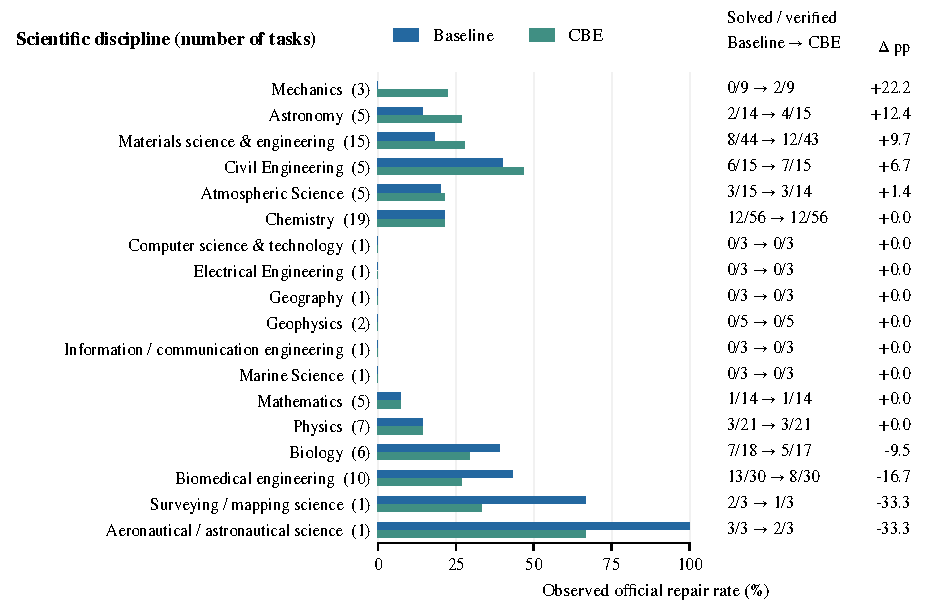
\includegraphics[width=\textwidth]{figures/domain_outcomes.pdf}
\captionof{figure}{Solve-rate difference (CBE $-$ Baseline) for the ten disciplines with non-zero change. Task counts in parentheses. Eight disciplines with identical solve rates across arms are omitted.}
\label{fig:domains}
\end{minipage}\vspace{9pt}}]

Figure~\ref{fig:domains} reveals a clean split beneath the aggregate parity. Six disciplines gain: mechanics (+22.2\,pp, entirely task 103), astronomy (+13.3\,pp, driven by sunpy), materials (+8.9\,pp across DeePTB, deepmd-kit, and dpdata), atmospheric science (+6.7\,pp), civil engineering (+6.7\,pp), and chemistry (+1.8\,pp). Four decline: biomedical engineering ($-$16.7\,pp across four tasks including nilearn), biology ($-$5.6\,pp across biopython and tskit), and the singletons surveying and aeronautical ($-$33.3\,pp each). The remaining eight disciplines, including physics (7 tasks) and mathematics (5), show zero difference.

\paragraph{Connection to task paradigms.}
The benchmark organizes tasks into three paradigms~\citep{xu2026science}. CBE marginally helps \emph{Issue-driven} tasks (+1.5\,pp), where localization matches the repair need; slightly hurts \emph{Expert-exploratory} tasks ($-$1.8\,pp), where indexed formulas anchor the agent instead of letting it reason about the anomaly; and has no effect on \emph{Engineering-integration} tasks (0\,pp), where multi-file architecture is the bottleneck. Of the benchmark's four failure mechanisms, CBE addresses the first (knowledge deficit) for computation tasks and triggers the second (anchoring) on interface tasks. It does not touch system integration or scientific generalization.

\paragraph{Replication.}
Baseline and CBE never solve 60 and 59 tasks, respectively. Outcomes are mixed on 18 baseline and 19 CBE tasks; 11 tasks succeed in all three runs for each arm. About a fifth of tasks flip between runs; the confidence interval ($[\CILower, \CIUpper]$\,pp) spans zero.

\paragraph{Implications for representation design.}
The zero-change disciplines --- physics (7), mathematics (5), and six singletons --- contain bugs in test infrastructure and configuration, not mathematical pipelines. A representation that also indexes interface contracts and configuration schemas might extend the benefit without anchoring.

\vspace{4pt}
\begin{minipage}{\columnwidth}
\centering
\begin{tikzpicture}[x=1mm,y=1mm,
  every node/.style={font=\fontsize{7.5}{9}\selectfont},
  box/.style={draw=baselineblue!60,fill=baselineblue!4,rounded corners=.8mm,align=center,minimum height=7mm,inner sep=1.5mm},
  arr/.style={-{Stealth[length=1.2mm]},draw=baselineblue!70,line width=.5pt}]
\node[box,text width=20mm] (a) at (0,0) {\textbf{Trace}\\reproducer};
\node[box,text width=20mm] (b) at (28,0) {\textbf{Extract}\\AST + CPG};
\node[box,text width=20mm] (c) at (56,0) {\textbf{Store}\\evidence};
\node[box,text width=20mm,draw=cbeteal!60,fill=cbeteal!4] (d) at (56,-12) {\textbf{Query}\\find / inspect / note};
\node[box,text width=20mm] (e) at (28,-12) {\textbf{Repair}\\edit + test};
\draw[arr] (a)--(b); \draw[arr] (b)--(c); \draw[arr] (c)--(d); \draw[arr] (d)--(e);
\end{tikzpicture}
\captionof{figure}{CBE pipeline: trace the reproducer, extract computation structure, store it, then the agent queries and repairs.}
\label{fig:method}
\end{minipage}

\clearpage
\twocolumn[{\begin{minipage}{\textwidth}
\section{Case studies}
\label{sec:cases}
\centering
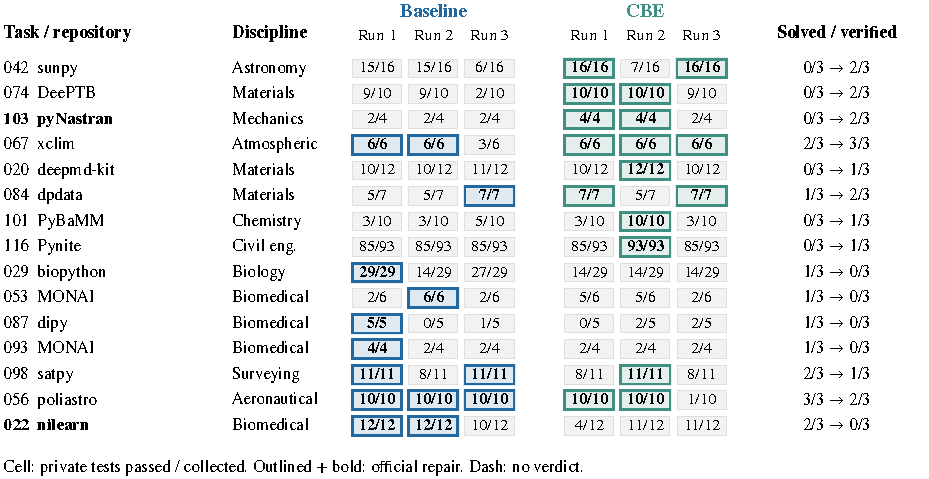
\includegraphics[width=\textwidth]{figures/trial_test_matrix.pdf}
\captionof{figure}{Per-run private-test pass fractions for every task whose solve rate differs between arms. Outlined bold cells are official solves; bold task labels are the two cases below.}
\label{fig:trials}
\vspace{3pt}
\captionof{table}{Comparison of generated patches for divergent case studies.}
\label{tab:cases}
{\fontsize{8}{9.5}\selectfont\setlength{\tabcolsep}{2.5pt}\renewcommand{\arraystretch}{1.05}
\begin{tabularx}{\textwidth}{@{}p{1.1cm}XXX@{}}
\toprule
Task & Baseline & CBE & Insight \\
\midrule
103 pyNas\-tran & Expand ply iteration; keep original B/D accumulation. All pass public. & Two fix both expansion and B/D; third keeps old accumulation. & Public check undertests. Full computation structure separates complete from partial repairs. \\
\addlinespace[1pt]
022 nilearn & Add label aggregation; preserve nearest-neighbour path. & Two alter argument handling (11/12 private); third fails (4/12). & Interface preservation is the obligation. CBE patches also alter existing arguments. \\
\bottomrule
\end{tabularx}}
\end{minipage}\vspace{2pt}}]

\paragraph{Task 103 (pyNastran).}
Figure~\ref{fig:trials} shows per-run outcomes. Baseline expands ply iteration but keeps original B/D accumulation; all pass public, all fail private. CBE exposes the accumulation formula; two of three attempts fix both expressions and pass.

\paragraph{Task 022 (nilearn).}
Baseline adds label aggregation while preserving the nearest-neighbour path. CBE attempts read coordinate-projection mathematics and alter argument handling --- passing 11/12 private tests but failing backward compatibility.

\section{Limitations and conclusion}
\label{sec:conclusion}
CBE extracts syntax, not semantics: function scopes, calculation expressions, conditions, and call boundaries from ASTs and code property graphs. It does not model domain meaning, inter-module behavioural contracts, or backward-compatibility invariants, and unresolved callees are labelled \texttt{unknown\_external} rather than inferred. The evaluation uses one model family and one scaffold, so the discipline split may not transfer to other agents. No component ablation separates the contribution of the reproducer trace, the expression index, or the query endpoints. The measured effect is small: 15 of 89 tasks differ, the interval spans zero, and about a fifth of tasks flip between identical runs, which bounds what any single-run comparison can resolve. 81 of 89 tasks are pure Python, so the C, C++, Fortran, and Cython frontends are only lightly exercised.

The consistent direction of the split is the useful finding: pre-computed computation structure helps when the repair obligation is a calculation, and misdirects when it is preserving an interface. A representation that indexes interface contracts and configuration schemas alongside computation flows is the next step.

\section{AI Assistance}
ChatGPT and Oh My Pi assisted with coding, debugging, analysis, and plotting. Code, receipts, and per-task outcomes: \url{https://github.com/rajarshighoshal/computation-boundary-evidence}.

\clearpage
\bibliography{references}
\end{document}
